\section{Príručka na používanie riešenia}
\label{sec:prirucka}

Zdrojový kód je archivovaný v repozitári GitHub~\cite{repo}.

% ----- Požiadavky -----
\subsection{Požiadavky}

\begin{itemize}
  \item Node.js a npm (vyvíjané s Node.js 24),
  \item Python 3 (vyvíjané s verziou 3.14),
  \item prehliadač s podporou \code{canvas} a \code{performance.now()}
        (testované v Microsoft Edge).
\end{itemize}

% ----- Inštalácia -----
\subsection{Inštalácia}

\begin{lstlisting}
# 1. Stiahnutie projektu
git clone https://github.com/tetianamohorian23/bsb-keystroke.git
cd bsb-keystroke

# 2. Klient (React)
npm install

# 3. Server (Python) vo vlastnom virtuálnom prostredí
cd backend
python -m venv .venv
.venv\Scripts\activate          # Windows
pip install -r requirements.txt
\end{lstlisting}

% ----- Spustenie -----
\subsection{Spustenie}

Server a klient sa spúšťajú v dvoch samostatných termináloch.

\begin{lstlisting}
# Terminál 1: server na http://127.0.0.1:8000
cd backend
.venv\Scripts\uvicorn main:app --reload

# Terminál 2: klient (adresu vypíše Vite, zvyčajne http://localhost:5173)
npm run dev
\end{lstlisting}

Vývojový server Vite presmeruje požiadavky na cestu \code{/api} na server
na porte 8000 (nastavenie v \code{vite.config.js}). Databáza
\code{backend/sessions.sqlite3} sa vytvorí automaticky pri prvom spustení.
Produkčná zostava klienta sa vytvorí príkazom \code{npm run build}
do priečinka \code{dist/}.

% ----- Postup pre účastníka -----
\subsection{Postup pre účastníka}

Aplikáciu otvorte na počítači alebo notebooku s fyzickou klávesnicou:
na telefóne a tablete sa zobrazí hlásenie „Nie je podporované“.
\begin{enumerate}
  \item Na úvodnej obrazovke zadajte meno a priezvisko, vyberte zariadenie
        a klávesnicu (pri stolovom počítači nie je ponuka „Vstavaná“),
        v poli „Čo budete písať“ zvoľte vetu alebo slovo a zaškrtnite súhlas.
        Tlačidlo „Začať meranie“ sa aktivuje až po vyplnení mena a súhlasu.
  \item Napíšte zobrazený text rovnako, ako bežne píšete, a potvrďte ho
        klávesom Enter. Backspace a Delete nefungujú: ich stlačenie aj
        nesprávny znak pokus nezapočítajú: vstup sa na chvíľu zamkne,
        zobrazený text sa zatrasie a hlásenie vysvetlí, čo sa stalo; potom
        písanie začnete odznova a počítadlo sa nezvýši. Pokus
        s neuvoľnenou klávesou sa nezapočíta.
  \item Po 15 správnych pokusoch sa zobrazí súhrn (počet pokusov, priemerná
        doba držania klávesy a priemerný čas napísania textu).
  \item Relácia sa na server uloží automaticky, tlačidlo na odoslanie nie je
        potrebné. Ak uloženie zlyhá, zobrazia sa tlačidlá „Skúsiť znova“
        a „Stiahnuť CSV“. Opakované odoslanie tej istej relácie sa nezapíše
        znova.
\end{enumerate}

% ----- Identifikácia pokusu -----
\subsection{Identifikácia pokusu}

Na úvodnej obrazovke tlačidlo „Rozpoznať pokus“ otvorí režim, v ktorom
účastník napíše zvolený text (vetu alebo slovo, podľa režimu zvoleného na
úvodnej obrazovke) jedenkrát. Server vráti troch najpodobnejších
účastníkov s relatívnou mierou podobnosti, alebo označí pokus ako neznámy.
Režim vyžaduje, aby v databáze existovali relácie s dostatočným počtom
platných pokusov.

Výsledok identifikácie na skutočných dátach ukazuje Obr.~\ref{fig:identify}: pokus napísal účastník, ktorého šablóna je v databáze, a server ho
priradil správne. Okrem najpodobnejšieho účastníka zobrazí aplikácia aj
ďalších dvoch kandidátov. Percentá udávajú len relatívne poradie medzi
troma najbližšími šablónami, nie pravdepodobnosť zhody.

% Obrázok (obrázok zo súboru figures/ui-identify.png): Identifikácia pokusu na skutočných dátach: najpodobnejší účastník a relatívna miera podobnosti troch najlepších kandidátov.
\begin{figure}[ht]
  \centering
  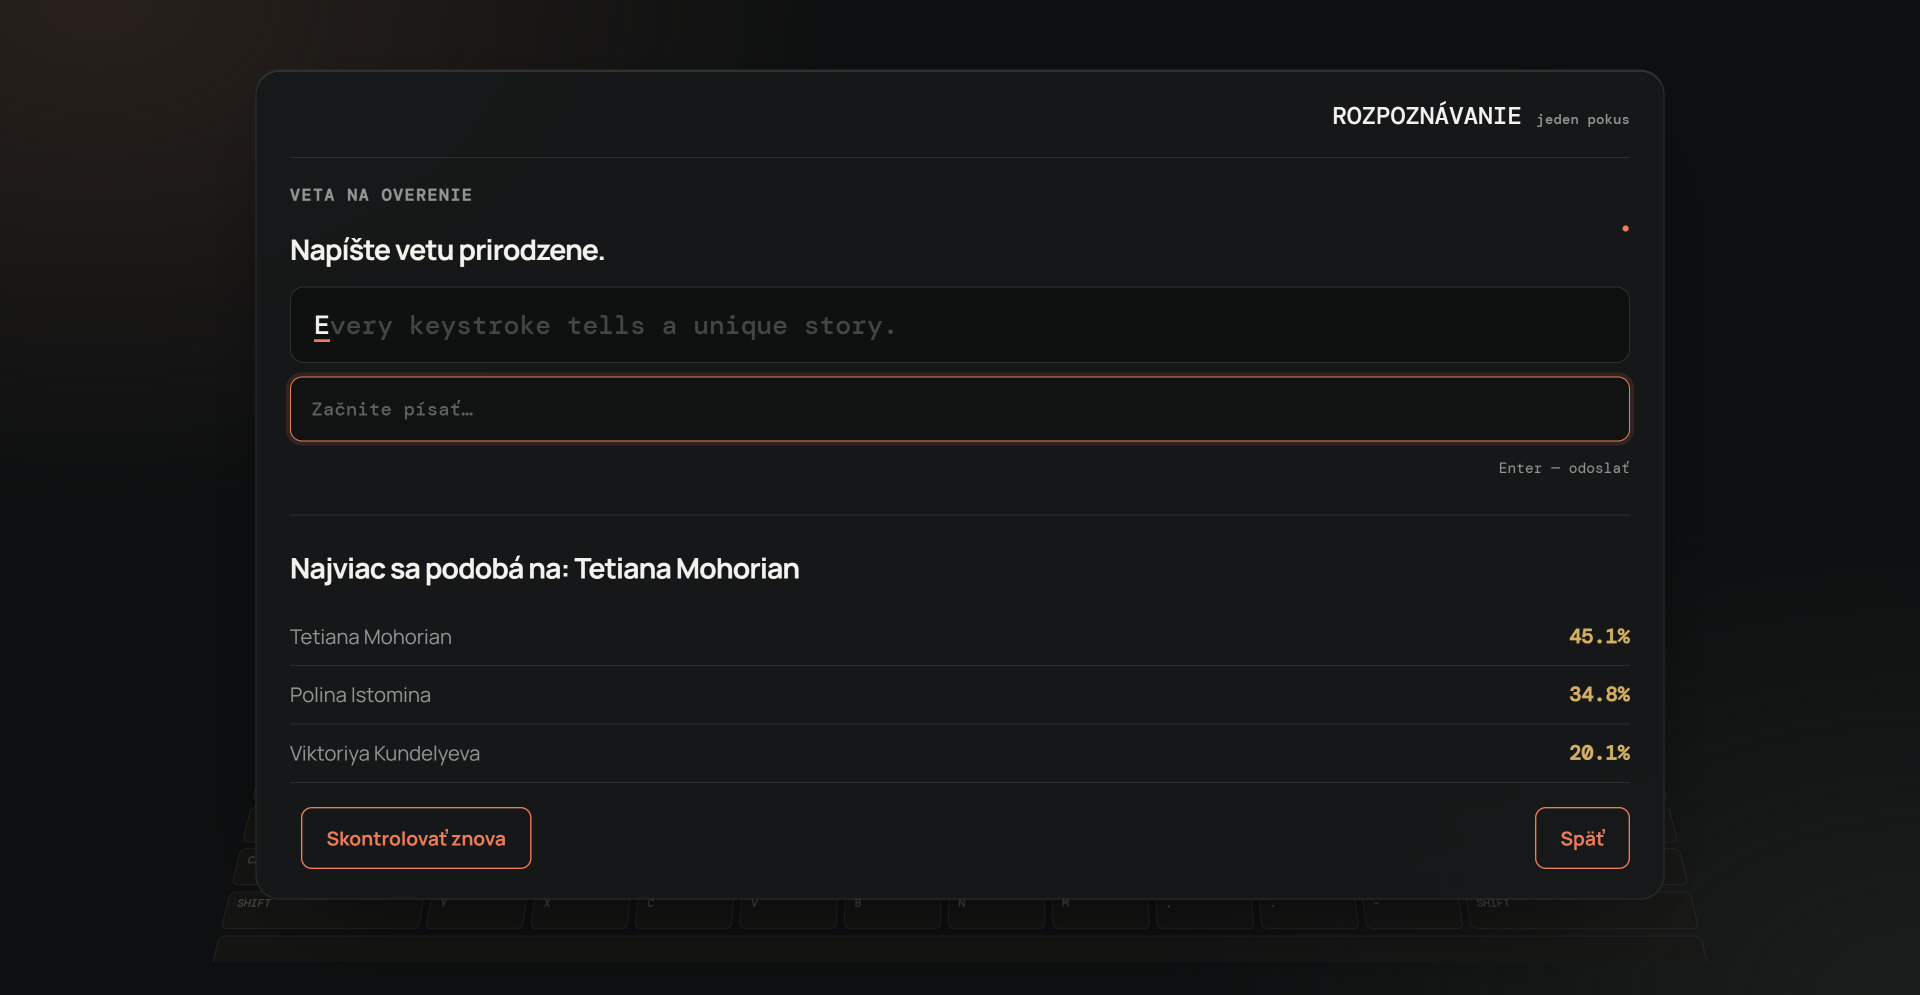
\includegraphics[width=\textwidth]{ui-identify.png}
  \caption{Identifikácia pokusu na skutočných dátach: najpodobnejší účastník
           a relatívna miera podobnosti troch najlepších kandidátov.}
  \label{fig:identify}
\end{figure}

% ----- Reprodukovateľnosť -----
\subsection{Reprodukovateľnosť}
\label{sec:prirucka-repro}

Verzie závislostí klienta zaisťuje súbor \code{package-lock.json}.
Databáza so zozbieranými dátami obsahuje osobné údaje, preto sa
nemá verzionovať; na reprodukciu vyhodnotenia je potrebné zozbierať nové dáta
(minimálne 10 pokusov na účastníka na tvorbu šablóny a 1 až 5 pokusov
na testovanie).
